\documentclass[10pt,a4paper]{article}
\usepackage[utf8]{inputenc}
\usepackage{amsmath}
\usepackage{amsfonts}
\usepackage{amssymb}
\usepackage{graphicx}
\usepackage[T1]{fontenc} 
\author{Michał Chilczuk\\Kateryna Saienko
\\Bartosz Frączak}
\title{Projekt WDEC - Symulacja gry rynkowej}
\begin{document}
\maketitle
\section{Zadanie}
Program ma za zadanie wspomaganie użytkownika w podejmowaniu decyzji w obrębie symulatora gry rynkowej. Gracz ma wpływ na takie wartości jak wielkość produkcji, jakość, wydatki na marketing. Zadaniem programu jest wspomożenie gracza w dobraniu powyższych wartości.
\section{Model}
Zastosowano 2 kryteria służące do oceny jakości decyzji:
\begin{itemize}
\item zysk - określony jako:
\begin{equation*}
\text{zysk} = \text{cena} \cdot \text{wielkość produkcji} - \text{koszt}(\text{wielkość produkcji})
\end{equation*}

gdzie, cena to dane z pola "Cena", wielkość produkcji to dane, które są pobrane z pola "Wolumen".
Natomiast dla kosztu produkcji istnieje następująca zależność:
\begin{equation*}
\text{koszt} = \text{koszt jednostkowy}(\text{wielkość produkcji},\text{jakość}) \cdot \text{wielkość produkcji}
\end{equation*}
Konieczne okazało się aproksymacja funkcji kosztu jednostkowego produktu zależnego od wielkości produkcji i jakości produktu. W tym celu zebrano kilkadziesiąt próbek sprawdzając jak koszt jednostkowy zmienia się dla różnych wartości. Okazało się, że zależność od wolumenu prezentuje się następująco.
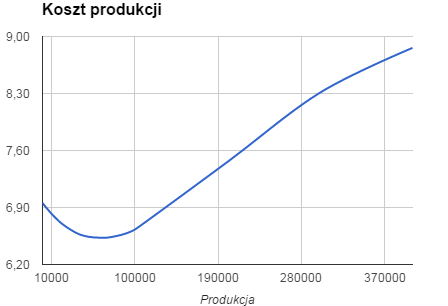
\includegraphics[scale=0.75]{koszt} \\
Jak widać dla małych wartości wolumenu funkcja jest malejąca, osiąga minimum a następnie gwałtownie rośnie.
\\
Ostatecznie otrzymano następującą funkcję aproksymującą koszt jednostkowy produktu:
\begin{multline*}
\text{koszt}(p,q) = -1.353 \cdot 10{-28} \cdot p^5 + 4.755 \cdot 10^{-22} \cdot p^4 - 4.408 \cdot 10^{-16} \cdot p^3 + 1.588 \cdot 10^{-10} \cdot p^2 \\
 - 1.518 \cdot 10^{-5} \cdot p + 6.954  \\
+ 1.474 \cdot 10^{-5} \cdot q^3- 1.87 \cdot 10^{-3} \cdot q^2+ 0.103 \cdot q -0.248
\end{multline*}

Prognozowany przychód definiowany jest jako iloczyn przewidywanej wielkości sprzedaży i zaproponowanej cany:
\begin{equation*}
\text{przychód} = \text{wielkość sprzedaży} \cdot \text{cena}
\end{equation*}

Natomiast całkowity koszt składa się z kosztu zmiennego zależnego od ceny i jakości oraz kosztu stałego.
\begin{equation*}
\text{koszt całkowity} = \text{wolumen} \cdot \text{koszt jednostkowy} + \text{koszt stały}
\end{equation*}

Zysk obliczany jest jako różnica powyższych wartości.
\begin{equation*}
\text{zysk} = \text{przychód} - \text{koszt całkowity}
\end{equation*}
\end{itemize}
\begin{itemize}
\item ryzyko - zdefiniowane jako:
\begin{equation*}
\text{ryzyko} = \frac{\text{popyt}}{\text{wielkość produkcji}}
\end{equation*}


Współczynnik ryzyka przyjmuje wartości od 0 do 1. Wartość 1 oznacza sprzedanie całego wyprodukowanego towaru, natmiast 0 całkowity brak sprzedaży. \\
Wartość tego współczynnika w różnym stopniu zależy od wszystkich zmiennych decyzyjnych. Po wykonaniu eksperymentów otrzymano wniosek, że największy wpływ na ryzyko mają jakość produkcji i cena. Dlatego zebrano dane przyjmując stały wolumen równy 5000 i różne wartości zmiennych jakości i ceny. Zebrane dane posłużyły do wyprowadzenia funkcji prognozującej sprzedaż produktu. Jest ona rozbita na dwa czynniki zależne od obu zmiennych:
\begin{itemize}
\item zależny od jakości
\begin{equation*}
7.932 \cdot 10^{-7} \cdot q^3 - 1.943 \cdot 10^{-4} \cdot q^2 + 0.019 \cdot q - 0.207;
\end{equation*}
\item zależny od ceny
\begin{equation*}
1.135 \cdot 10^{-3} \cdot p^2 + 0.035 \cdot p + 0.1;
\end{equation*}
\end{itemize}
Z ich pomocą obliczana jest prognoza sprzedaży korzystając z następującego wzoru:
\begin{equation*}
\text{prognoza sprzedaży} = (1-\text{czynnik ceny}+\text{czynnik jakości}) \cdot \text{zapotrzebowanie}
\end{equation*}
gdzie zapotrzebowanie jest prognozowanym popytem produktu sczytanym z symulatora.
Następnie z użyciem otrzymanej wartości otrzymywane jest ryzyko.
\begin{equation*}
\text{ryzyko} = \frac{\text{prognoza sprzedaży}}{\text{wielkość produkcji}}
\end{equation*}
\end{itemize}
\section{Działanie programu}
Użytkownik wprowadza zmienne decyzyjne a także wartość prognozowanego popytu podaną przez symulator. Program przelicza podane wartości zwracając następujące wielkości:
\begin{itemize}
\item koszt zmienny jednostkowy produktu
\item prognozowany przychód
\item przewidywany koszt całkowity
\item zysk
\item ryzyko
\end{itemize}
Oprócz tego rysuje wykresy kryteriów decyzyjnych (zysku i ryzyka) w zależności od wolumenu produkcji.
Ułatwia to użytkownikowi podjęcie prawidłowej decyzji.
\section{Prezentacja interfejsu aplikacji}
Główne okno programu prezentuje się następująco:\\
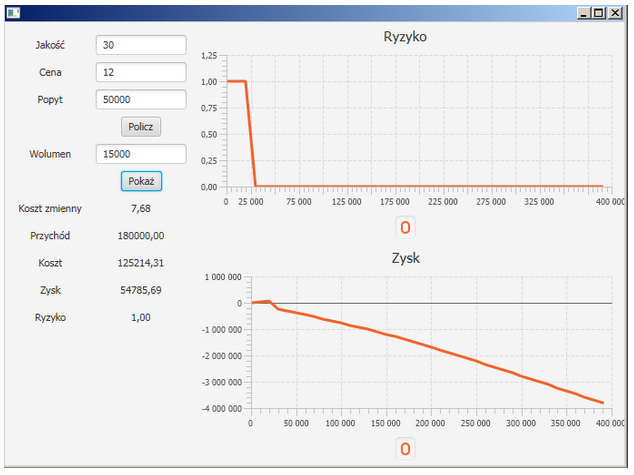
\includegraphics[scale=0.75]{screen}
\end{document}
